\subsection{Physikalische Grundlagen}
Die Gleichungen und Erklärungen dieses Kapitels beruhen auf \cite{herrmann}.
\subsubsection{Faraday-Effekt}
Der \emph{Faraday-Effekt} tritt auf, wenn linear polarisiertes Licht durch ein isotropes Medium, welches mit ein Magnetfeld in 
Ausbreitungsrichtung des Lichts durchflossen ist, propagiert. Das Magnetfeld verursacht eine zirkulare Doppelbrechung, das heißt links- und 
rechtsdrehende elektromagnetische Wellen haben einen unterschiedlichen Brechungsindex. \\
Da linear polarisiertes Licht als Überlagerung von zwei, in entgegengesetzter Richtung zirkular polarisierten elektromagnetischen Wellen 
beschrieben werden kann, eilt eine Welle der anderen voraus und das Licht, welches das Medium durchläuft, wird um einen Winkel $\alpha$ gedreht. 
Die Stärke der Drehung hängt proportional von der magnetischen Feldstärke $H$ der Spule ab, welche das Magnetfeld erzeugt. 
Dies bedeutet, dass bei Umkehrung des Spulenstroms, was einer Umpolung entspricht, das Licht in entgegengesetzte Richtung gedreht wird. 
Die Drehung ist also nicht reversibel, spiegelt man das Licht und lässt es das Medium in anderer Richtung durchqueren, 
so verdoppelt sich die Drehung\footnote{Im Gegensatz zu optisch aktiven Substanzen, die eine ausgezeichnete Drehrichtung haben 
und die erste Drehung rückgängig machen.}. Weiterhin hängt der Drehwinkel $\alpha$ proportional von der Länge $l$ des Mediums ab.
Es gilt also:
\begin{equation}
\label{eq:faraday}
  \alpha = V \cdot l \cdot H
\end{equation}
wobei $V$ eine Materialkonstante, auch \emph{Verdet-Konstante} genannt, ist.

\subsubsection{Bestimmung der magnetischen Feldstärke einer Zylinderspule}
\paragraph{Gesetz von Biot-Savart}
Die magnetische Flussdichte $\difd \vec{B}$ am Ort $\vec{r}$ eines mit dem Strom $I$ durchflossenen Leiters mit Länge $\difd \vec{l}$ 
am Ort $\vec{r}'$ lässt sich mit Hilfe des \emph{Biot-Savart}-Gesetzes bestimmen:
\begin{equation}
  \label{eq:biotsavart}
  \difd \vec{B}(\vec{r}) = \frac{\mu_0 \cdot I}{4 \pi} \cdot \difd \vec{l} \times \frac{\vec{r} - \vec{r}'}{\abs{\vec{r} - \vec{r}'}^3}
\end{equation}
\paragraph{Kreisförmige Leiterschleife}
Es wird zuerst eine kreisförmige Leiterschleife parallel zu der $x$-$y$-Ebene mit dem Radius $R$ betrachtet (\autoref{img:circloop}) \cite{dem2}.
\begin{figure}[H]
\begin{center}
  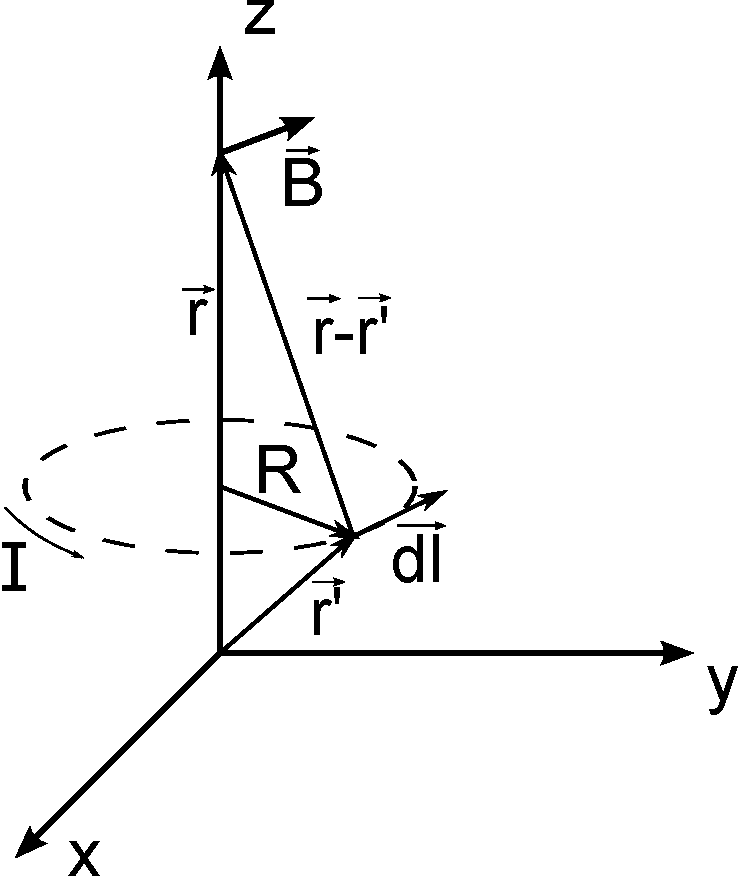
\includegraphics[width=0.3\textwidth]{../img/circloop.pdf}
  \caption{Kreisförmige Leiterschleife mit Radius $R$, parallel zur $x$-$y$-Ebene.}
  \label{img:circloop}
\end{center}
\end{figure}

Da die Komponente $\difd B_\perp = \difd B \cdot \sin \alpha$ senkrecht zur $z-$Achse bei der Integration über $\difd l$ verschwindet 
(Rotationssymmetrie), bleibt es nur die parallele Komponente $\difd B_\parallel = \difd B \cdot \cos \alpha$ zu betrachten. Wie in 
\autoref{img:bvector} zu erkennen ist, gilt
\begin{equation}
\label{eq:absdif}
  \abs{\difd \vec{l} \times \left( \vec{r} - \vec{r}' \right)} = \abs{\vec{r} - \vec{r}'} \cdot \difd l \cdot \underbrace{\sin \varphi}_{= 1} 
  = \abs{\vec{r} - \vec{r}'} \cdot \difd l = \frac{R}{\cos \alpha} \cdot \difd l
\end{equation}
\begin{figure}[H]
\begin{center}
  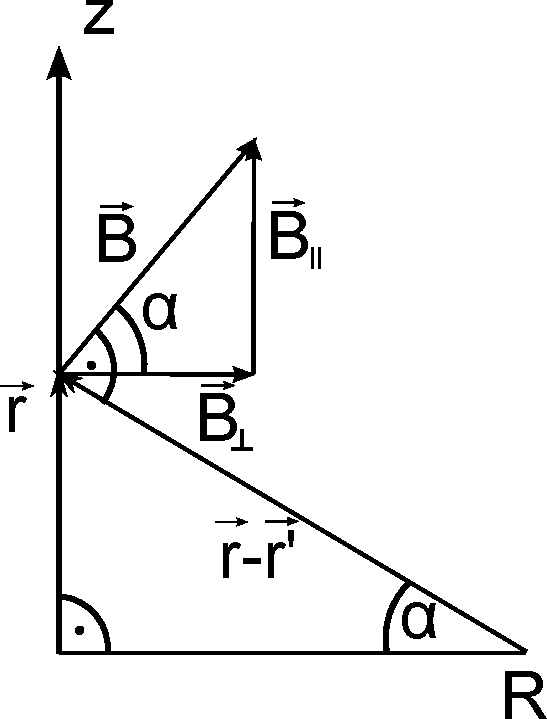
\includegraphics[width=0.3\textwidth]{../img/bvector.pdf}
  \caption{Komponenten des $\vec{B}$-Vektors und Dreieck zwischen $R$, $\vec{r}-\vec{r}'$ und $\vec{r}$.}
  \label{img:bvector}
\end{center}
\end{figure}
Es folgt für $B_\parallel$:
\begin{equation}
\begin{split}
  \label{eq:bparallel}
    B_\parallel &= \int \difd B_\parallel = \int \difd B \cdot \cos \alpha \\
  &\refeq{eq:faraday} \frac{\mu_0 \cdot I}{4 \pi} \cdot \oint \frac{\abs{\difd \vec{l} \times \left( \vec{r} - \vec{r}' \right)}}{\abs{\vec{r} - \vec{r}'}^3} \cdot \cos \alpha \\
  &\refeq{eq:absdif} \frac{\mu_0 \cdot I}{4 \pi} \cdot \frac{R}{\abs{\vec{r} - \vec{r}'}^3} \cdot \oint \difd s = \frac{\mu_0 \cdot I}{2} \cdot \frac{R^2}{\abs{\vec{r} - \vec{r}'}^3}
\end{split}
\end{equation}
Mit $\abs{\vec{r} - \vec{r}'}^2 = R^2 + (z-z')^2$ folgt damit für die magnetische Flussdichte $\vec{B}_K(z, z')$
\begin{equation}
  \vec{B}_K(z, z') = B_\parallel \cdot \hat{e}_z \refeq{eq:bparallel} \frac{\mu_0 \cdot I}{2} \cdot \frac{R^2}{ \left( R^2 + (z-z')^2 \right)^{3/2}} \cdot \hat{e}_z
\end{equation}
Die magnetische Feldstärke $H_K$ ist also
\begin{equation}
  H_K(z, z') = \frac{B_K(z, z')}{\mu_0} = \frac{I}{2} \cdot \frac{R^2}{ \left( R^2 + (z-z')^2 \right)^{3/2}}
\end{equation}
\paragraph{Reale Zylinderspule}
Eine reale Zylinderspule der Länge $L$ besitzt einen Innen- und Außenradius ($r_i$ und $r_a$). 
Weiterhin wird angenommen, dass die Windungen $N$ homogen gewickelt sind. Daher gilt für die differentielle Windugszahl $\difd N$ in einem 
Rechteck mit Seiten $\difd z'$ und $\difd R$:
\begin{equation}
  \difd N = \frac{N}{L} \cdot \difd z' \cdot \frac{\difd R}{r_a - r_i}
\end{equation}
Für das Magnetfeld $H(z)$ der realen Spule folgt nun \cite{herrmann}:
\begin{equation}
  \label{eq:hreal}
  \begin{split}
    H(z) &= \frac{N}{L} \cdot \int_{r_i}^{r_a} \frac{\difd R}{r_a - r_i} \cdot \int_{0}^{L} B_K(z, z')\, \difd z'\\
    &=\frac{N \cdot I}{2 L \left( r_a - r_i \right) } \cdot \left[ 
  	      (L-z) \cdot \ln \left( \frac{r_a + \sqrt{(L-z)^2  +r_a^2}}{r_i + \sqrt{(L-z)^2 + r_i^2}} \right) + 
  		  z \cdot \ln \left( \frac{r_a + \sqrt{z^2  +r_a^2}}{r_i + \sqrt{z^2 + r_i^2}} \right)  \right]
  \end{split}
\end{equation}
\subsubsection{Bestimmung des Drehwinkels in Abhängigkeit des Stroms}
\label{subsub:alpha}
Das Licht wird nun nach \autoref{eq:faraday} pro Wegstrecke $\difd z$ um folgenden Winkel $\difd \alpha$ gedreht:
\begin{equation}
  \difd \alpha = V \cdot H(z) \cdot \difd z
\end{equation}
Der gesamte Winkel $\alpha$ berechnet sich mit den gegebenen Werten \cite{manual} für diesen Versuch zu:\footnote{Mit Mathematica berechnet.}
\begin{equation}
  \label{eq:verdet}
  \alpha = V \int_{\frac{L-l}{2}}^{\frac{L+l}{2}} H(z)\, \difd z = 2554.85 \cdot V \cdot I 
\end{equation}